% !TEX root = ./QF_A-Lab.1.tex
\providecommand\mainfilename{"./QF_A-Lab.tex"}
\providecommand \subfilename{}
\renewcommand   \subfilename{"./QF_A-Lab.1.tex"}
\documentclass[\mainfilename]{subfiles}

% \tikzset{external/force remake=true} % - remake all

\begin{document}

\graphicspath{{\subfix{./.build/figures/QF_A-Lab.1}}}
\tikzsetexternalprefix{./.build/figures/QF_A-Lab.1/}

\mymakesubfile{1}
[QF A]
{Laboratório -- CMC: Concentração Micelar Crítica} % Subfile Title
{Laboratório -- CMC: Concentração Micelar Crítica} % Part Title

\part*{Introdução}

\begin{sectionBox}1{Du Noüy Ring Method} % S1
    
    \begin{BM}
        \gamma_{ap}=\frac{M\,g}{4\,\pi\,R}f
    \end{BM}

    \begin{description}[
        leftmargin=!,
        labelwidth=\widthof{M} % Longest item
    ]
       \item[M] é o peso máximo do líquido levantado acima da superfície do líquido
       \item[g] é a constante gravitacional (\qty{9.780327}{\metre/\second^2})
       \item[R] é o raio do anel de platina
       \item[F] é o fator de correção
    \end{description}

    \paragraph*{O fator de correção} depende das dimensões do anél e pode ser determinado por intermédio das tabelas dependendo de:
    \begin{itemize}
        \begin{multicols}{2}
            \item Raio do anél
            \item Raio do fio
            \item densidade do líquido
            \item Temperatura
        \end{multicols}
    \end{itemize}
    
\end{sectionBox}

\begin{sectionBox}1{Equação de Young} % S2
    
    \begin{BM}
        \gamma_{s.v} 
        = \gamma_{s.l} 
        + \gamma_{l.v}\,\cos{\theta}
        \\
        \begin{cases}
            \theta=0 & \text{(Liq molha completamente o sólido)}
            \\0<\theta<\pi/2 &\text{(Liq molha parcialmente o sólido)}
            \\\theta\geq\pi/2 &\text{(Liq não molha a superfície)}
        \end{cases}
    \end{BM}

    \begin{multicols}{2}
        \begin{description}[
            leftmargin=!,
            labelwidth=\widthof{} % Longest item
        ] 
            \item[\(\gamma\)] Energia Interfacial
            \item[\(\theta\)] Angulo de contato
        \end{description}

        \vspace{1ex}
    
        \begin{description}[
            leftmargin=!,
            labelwidth=\widthof{s.v} % Longest item
        ]
            \item[\(s.v\)] solido--vapor
            \item[\(s.l\)] solido--liquido
            \item[\(l.v\)] liquido--vapor
        \end{description}
    \end{multicols}

    
\end{sectionBox}

\begin{sectionBox}1{Trabalho de adesão (Dupré)} % S3
    
    \begin{BM}
        W_{s.l}=\gamma_{s.v}+\gamma_{l.v}-\gamma_{s.l}
    \end{BM}

    \subsection*{Equação de Young--Dupré}
    \begin{BM}
        W_{s.l}=\gamma_{l.v}(1+\cos{\theta})
    \end{BM}\vspace{-4ex}
    \begin{flalign*}
        &
            W_{s.l}
            = \gamma_{l.v}+\gamma_{s.v}-\gamma_{s.l}
            = \gamma_{l.v}+\gamma_{l.v}\,\cos{\theta}
            = \gamma_{l.v}(1+\cos{\theta})
        &
    \end{flalign*}
    
\end{sectionBox}

\part*{Dados}

% \tikzset{
%     every axis plot/.append style={}
% }

\begin{sectionBox}1{Tensão Superficial} % S
    
    \begin{center}
        \vspace{1ex}
        \begin{tabular}{*{4}{C}}

            \toprule
            
                \ch{[SDS]}/\unit{M}
                & \ln\ch{[SDS]}/\unit{M}
                & \multicolumn{1}{c}{T. Sup 1}
                & \multicolumn{1}{c}{T. Sup 2}
            
            \\\midrule

            \multicolumn{4}{l}{Concentrações teóricas}

            \\\midrule

                5.00\E-04 & \num{-7.60090246}  & 40.88 & 40.75
            \\  1.00\E-03 & \num{-6.907755279} & 33.37 & 33.44
            \\  5.00\E-03 & \num{-5.298317367} & 26.65 & 26.87
            \\  8.00\E-03 & \num{-4.828313737} & 22.52 & 27.85
            \\  2.00\E-02 & \num{-3.912023005} & 28.03 & 28.22
            \\  3.00\E-02 & \num{-3.506557897} & 28.65 & 28.83
            \\  5.00\E-02 & \num{-2.995732274} & 29.05 & 29.22

            \\\midrule

            \multicolumn{4}{l}{Concentrações reais}

            \\\midrule
            
                5.05\E-04 & \num{-7.590952129} & 40.88 & 40.75
            \\  1.01\E-03 & \num{-6.897804948} & 33.37 & 33.44
            \\  5.05\E-03 & \num{-5.288367036} & 26.65 & 26.87
            \\  8.08\E-03 & \num{-4.818363406} & 22.52 & 27.85
            \\  2.02\E-02 & \num{-3.902072675} & 28.03 & 28.22
            \\  3.03\E-02 & \num{-3.496607566} & 28.65 & 28.83
            \\  5.05\E-02 & \num{-2.985781943} & 29.05 & 29.22

            \\\bottomrule
        \end{tabular}
        \\[1ex]\tablecaption{Tensões superficiais adquiridas no laboratório}
        \vspace{2ex}
    \end{center}

    \begin{center}
        \begin{figure}
        \tikzset{external/force remake=true}
        %\pgfplotsset{height=7cm, width= .6\textwidth}
        % {\Large\bfseries{}}\par\medskip
        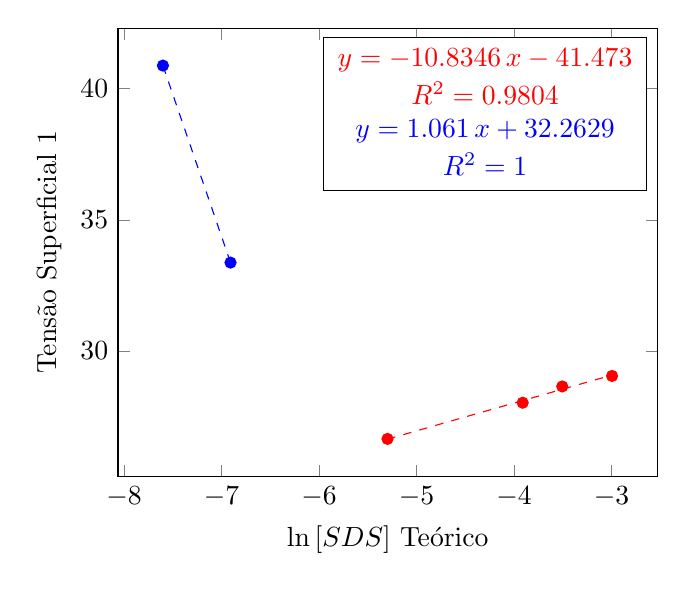
\begin{tikzpicture}
        \begin{axis}[
            xlabel={\(\ln{\ch{[SDS]}}\) Teórico},
            ylabel={Tensão Superficial 1},
        ]
            % Legends
            \addlegendimage{empty legend}
            \addlegendentry[red\Light]{\(y=-10.8346\,x-41.473\)}
            \addlegendimage{empty legend}
            \addlegendentry[red\Light]{\(R^2=0.9804\)}

            \addlegendimage{empty legend}
            \addlegendentry[blue\Light]{\(y=1.061\,x+32.2629\)}
            \addlegendimage{empty legend}
            \addlegendentry[blue\Light]{\(R^2=1\)}

            \addplot[
                no marks,
                dashed,
                draw=blue\Light,
            ] expression[
                domain=-7.6:-6.9
            ] {
                -10.8346*x-41.473
            };

            \addplot[
                mark=*,
                only marks,
                color=blue\Light,
                mark options={
                    fill=blue\Light,
                    fill opacity=1
                },
            ] coordinates {
                (-7.60090246 ,40.88)
                (-6.907755279,33.37)
            };

            \addplot[
                no marks,
                dashed,
                draw=red\Light,
            ] expression[
                domain=-5.3:-2.99
            ] {
                1.061*x+32.2629
            };

            \addplot[
                mark=*,
                only marks,
                color=red\Light,
                mark options={
                    fill=red\Light,
                    fill opacity=1
                },
            ] coordinates {
            (-5.298317367,26.65)
                (-3.912023005,28.03)
                (-3.506557897,28.65)
                (-2.995732274,29.05)
            };
            
        \end{axis}
        \end{tikzpicture}
        % \caption{}
        \end{figure}
    \end{center}
    
    Para encontrar a concentração micelar crítica, plotamos duas (supostas) retas, uma gravemente inclinada e uma aproximadamente horizontal, então tentamos achar o valor de \(\ln\ch{[SDS]}_f\) do conjunto horizontal na reta da curva inclinada:

    \begin{flalign*}
        &
            \text{CMC}
            = \exp{
                \frac{
                    \ln\ch{[SDS]}_f
                    + 41.473
                }{
                    -10.8346
                }
            }
            \cong \exp\left(
                \frac{
                    \frac{
                        28.03
                        + 28.65
                        + 29.05
                    }{3}
                    + 41.473
                }{
                    -10.8346
                }
            \right)
            \cong \num{0.001556419751695}
        &
    \end{flalign*}
    
\end{sectionBox}

\end{document}